\chapter{Simulations}
\label{cha:simulations}

This chapter is about the different simulations available with
SimSpark. In particular the soccer simulation is described in detail.

\section{The Soccer Simulation}
\label{sec:soccersimulation}

\subsection{Overview}

We implemented a simulation for SimSpark where two teams of up to 6
humanoid robots play soccer against each other. This seemingly simple
setup poses a challenge to agent implementers on several levels.

In order to act in a meaningful way on the playing field the first
challenge is to localize your agent on the playing field. To support
this the agents perceive their relative position to a set of
landmarks, called \texttt{flags} on the playing field. These flags
mark corner and goal spots of the playing field. Further the relative
location of other players and the ball are perceived.

If an agent knows where it is and where it wants to be in the near
future the next challenge is to walk there. The structure of the
humanoids are sufficiently realistic to make this non trivial. Further
the agent has to recover and get up if fallen over.

Another challenge is kicking the ball. As trivial this sounds to a
human it is far from trivial for a robot to keep its dynamic balance
when kicking and controlling the direction of the ball.

Agents that are able to move and kick the ball need to cooperate and
form a team. Only the effective application of strategic and
cooperative behaviors forms a successful team.

Most rules of the soccer game are judged by an automatic rule set that
enforces the basic soccer rule set. However more involved situations
like detection unfair behavior still require a human referee.

This soccer simulation is also used as the official competition environment for the 3D Soccer Simulation League at RoboCup\footnote{For more information on RoboCup, see also \url{http://www.robocup.org/}} \cite{KAK+97}\cite{KA00}\cite{BMO+05}\cite{MBS+07}. The robots used in the simulation at the competitions is the Soccerbot as described in chapter \ref{cha:robots}.

\begin{figure}[htp]
  \centering
  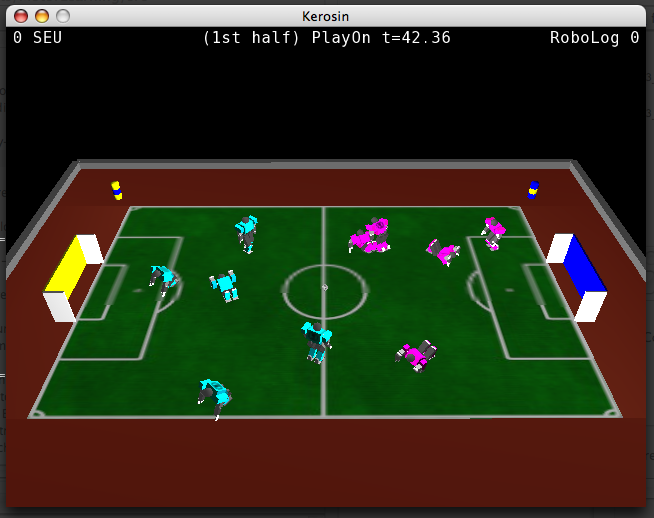
\includegraphics[width=\textwidth]{fig/soccersim}
  \caption{A screen shot of the soccer simulation with 5 vs 5 robots}
  \label{fig:soccersim}
\end{figure}

\subsection{Environment and Objects on the Field}

The dimensions of the soccer field are 18 by 12 meters. The center
spot has a radius of 4.5 meters. Each goal is 2.1 by 0.6 meter with a
height of 0.8 meters. The soccer field is surrounded by a border of 10
meters in each direction. Space outside this border area is not
reachable by an agent. The soccer ball has a radius of 0.04 meter and a
mass of 26 grams.

At each corner of the soccer field, and at the goal posts, a distinctive
flag is placed. The positions of these flags are fixed and known to
each agent. Agents perceive the relative position of a subset of
these flags and are therefore able to localize themselves on the soccer
field. The corner flags are color coded in the visualization. Agents
distinguish flags through their code name as shown in figure
\ref{fig:pitch}.

\begin{figure}[htp]
  \centering
  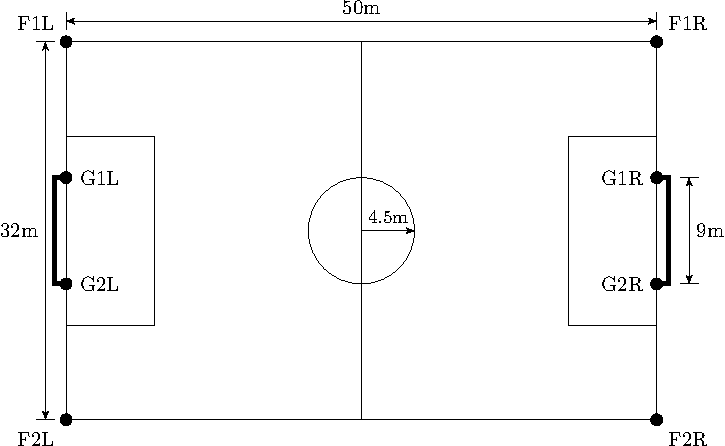
\includegraphics[width=\textwidth]{fig/pitch}
  \caption{The dimensions of the soccer pitch and the object markers on the field as perceived by an agent}
  \label{fig:pitch}
\end{figure}

\subsection{Rules Judged by the Automatic Referee}

The automatic referee automatically limits the time of each game
half. It further keeps track which player was the last one to touch
the ball and checks whether the ball enters the goal penalty areas of
the soccer field. 

It detects and scores \texttt{goals}, it automatically judges
\texttt{ball out} and gives a kick in or corner kick in to the correct team. 
The \texttt{offside} rule is implemented but still experimental.

\subsection{Rules Judged by the Human Referee}

The human referee acts through a connected monitor. It is responsible
to give the \texttt{kick off} command to start each game half. The
automatic referee currently does not resolve situations where the game
got stuck if for example several player block each other and no one is
able to reach the ball. Further it does not detect fouls like the use
of hands or otherwise behavior on the soccer field.

In these cases the human referee can \texttt{drop ball} the ball,
i.e. put it on a random location on the playing field to unstuck the
game. He is further able to command a \texttt{free kick} where one
player is able to shoot from a short distance to the goal.

%\subsection{Setup Script}


%%% Local Variables: 
%%% mode: latex
%%% TeX-master: "user-manual"
%%% End: 
